\documentclass[twoside]{article}
\input{ISC18-english.sty}

\begin{document}
	\thispagestyle{empty}
	
	%%%%%%%%%%%%%%%%% Article title header  %%%%%%%%%%%%%%%%%%%%
	\fancyhead[LE]{A Functional Beta Regression Approach for Analyzing Bounded Data}
	
	%%%%%%%%%%%%%%%%% Article authors header   %%%%%%%%%%%%%%%%%%%%
	\fancyhead[RO]{H. Dehnavi, et al.}
	
	\begin{center}
		{
\includegraphics [height=25mm, width=150.3mm] {Images/isc18E}} \\
		\vspace*{-1.8cm}
		
		\vspace*{4cm}
		
		%%%%%%%%%%%%%%%%% Updated Title for Conference %%%%%%%%%%%%%%%%%%%%
		{\Large \bf A Functional Beta Regression Approach for Analyzing Bounded Data with Derivative Information}\\
		
		%%%%%%%%%%%%%%%%% Article authors and affiliations %%%%%%%%%%%%%%%%%%%%
		{\bf
			Hamideh Dehnavi$^{1}$,
			Davood Shahsavani$^{1}$\footnote{{\bf Corresponding Author:} {\tt dshasavani@shahroodut.ac.ir}},
			Mohammad Arashi$^{2}$,
			Mohammad Fayaz$^{3}$ \\
			[6pt]
			$^{1}$Department of Statistics, Faculty of Mathematical Sciences, Shahrood University of Technology, Shahrood, Iran \\
			$^{2}$Department of Mathematics, Ferdowsi University of Mashhad, Mashhad, Iran \\
			$^{3}$School of Medicine, Shahed University, Tehran, Iran
		}
		
	\end{center}
	
	\rule{\textwidth}{0.2mm}\\
	
	\begin{abstract}
		This paper proposes a novel partial functional beta regression model for bounded responses in $(0,1)$. The model incorporates a functional predictor, its derivative, and additional scalar covariates, using a logit link function to model the mean of the beta distribution. We employ basis expansions and penalized maximum likelihood for estimation, capturing both global effects and dynamic behavior via the derivative term. Under standard regularity conditions, we establish the identifiability and consistency of the estimators. Simulation results and an application to near-infrared milk spectra demonstrate that integrating derivative information significantly improves predictive accuracy and provides better interpretability compared to standard functional models.
	\end{abstract}
	
	\noindent\textbf{Keywords:} beta regression; functional data analysis; derivative effects; penalized likelihood; NIR spectroscopy.
	
\section{Introduction}

In many modern scientific inquiries, statistical modeling is challenged by the simultaneous presence of bounded response variables and high-dimensional functional predictors. Traditional functional linear models \citep{Cardot1999} are designed for unrestricted continuous responses, making them theoretically and practically inadequate when the response represents a rate, proportion, or probability restricted to the interval $(0, 1)$. In such scenarios, ignoring the bounded nature of the response or applying standard Gaussian regression can lead to severe issues, including out-of-bound predictions and heteroscedasticity.

To address this limitation, beta regression \citep{FerrariCribari2004} has emerged as the standard framework for modeling bounded variables, offering a highly flexible mean--precision parameterization. While classical beta regression is well established for scalar covariates, its extension to functional predictors is still in its infancy. A notable advancement was made by \citet{DiBrisco2023}, who introduced a Bayesian flexible beta regression with functional covariates. However, most existing functional beta regression frameworks treat the functional predictor as a static curve, thereby overlooking the valuable dynamic information hidden within the trajectory's rate of change.

In practice, the derivative of a functional covariate often contains critical signals that are completely absent in the raw trajectories. For example, in near-infrared (NIR) spectroscopy, local slopes and rates of absorption carry physical meaning that can outperform raw intensity measurements. Incorporating derivative information in functional regression has strong theoretical and empirical support \citep{HallHooker2016, HookerShang2020}. Yet, despite its clear advantages, a unified, likelihood-based partial functional beta regression model that simultaneously integrates a functional predictor, its derivative, and additional scalar covariates has not yet been explored.

This paper fills this gap by proposing a novel partial functional beta regression framework. By employing basis expansions and penalized maximum likelihood estimation, our approach captures both the global impact of the curves and their fine-scale dynamic behavior via derivative information. The main contributions of this work are summarized as follows:
\begin{itemize}[leftmargin=1.2em]
	\item We introduce a novel partial functional beta regression model that accommodates a functional predictor, its first derivative, and scalar covariates.
	\item We develop a computationally efficient estimation scheme based on B-spline basis expansion combined with a penalized maximum likelihood approach to ensure smoothness.
	\item We establish the theoretical identifiability and consistency of the proposed estimators under standard regularity conditions.
	\item We demonstrate the superior predictive performance and interpretability of our model through extensive simulation studies and a real-world application to NIR milk spectroscopy data.
\end{itemize}

\section{Model formulation}
	
	Let $Y_i\in(0,1)$ denote the response for subject $i=1,\dots,n$. We assume
	\[
	Y_i \sim \mathrm{Beta}(\mu_i\phi,(1-\mu_i)\phi),
	\]
	where $\mu_i\in(0,1)$ is the mean and $\phi>0$ is a precision parameter. The beta density can be written as
	\[
	f(y_i\mid \mu_i,\phi)=
	\frac{\Gamma(\phi)}{\Gamma(\mu_i\phi)\Gamma((1-\mu_i)\phi)}
	y_i^{\mu_i\phi-1}(1-y_i)^{(1-\mu_i)\phi-1}, \qquad 0<y_i<1.
	\]
	
	We connect the mean to predictors through the logit link:
	\[
	\eta_i=\log\left(\frac{\mu_i}{1-\mu_i}\right)
	= \beta_0 + \int_{\T}\beta(t)X_i(t)\,dt
	+ \int_{\T}\alpha(t)X_i'(t)\,dt
	+ Z_i^\top\delta,
	\]
	where $X_i(t)$ is a functional predictor on $\T=[a,b]$, $X_i'(t)$ is its derivative, $Z_i$ is a vector of scalar covariates, and $\beta(t)$ and $\alpha(t)$ are unknown coefficient functions.
	
	The mean is therefore
	\[
	\mu_i = \frac{\exp(\eta_i)}{1+\exp(\eta_i)}.
	\]
	
	\subsection{Basis representation}
	
	To obtain a finite-dimensional model, we expand the coefficient functions in a basis $\{\psi_k(t)\}_{k=1}^K$:
	\[
	\beta(t)=\sum_{k=1}^K b_k\psi_k(t), \qquad
	\alpha(t)=\sum_{k=1}^K c_k\psi_k(t).
	\]
	Then
	\[
	\eta_i=\beta_0+\sum_{k=1}^K b_k \int_{\T}\psi_k(t)X_i(t)\,dt
	+\sum_{k=1}^K c_k \int_{\T}\psi_k(t)X_i'(t)\,dt
	+Z_i^\top\delta.
	\]
	Let
	\[
	x_{ik}=\int_{\T}\psi_k(t)X_i(t)\,dt,\qquad
	x'_{ik}=\int_{\T}\psi_k(t)X_i'(t)\,dt.
	\]
	In vector form,
	\[
	\eta_i=\beta_0+\mathbf{x}_i^\top\mathbf{b}+{\mathbf{x}_i'}^\top\mathbf{c}+Z_i^\top\delta.
	\]
	
	\subsection{Penalized likelihood estimation}
	
	Let $\theta=(\beta_0,\mathbf{b}^\top,\mathbf{c}^\top,\delta^\top,\phi)^\top$. The log-likelihood is
	\[
	\ell(\theta)=\sum_{i=1}^n \log f(y_i\mid \mu_i,\phi).
	\]
	To enforce smoothness of $\beta(t)$ and $\alpha(t)$, we maximize the penalized log-likelihood
	\[
	\ell_P(\theta)=\ell(\theta)
	-\lambda_\beta \mathbf{b}^\top S_\beta \mathbf{b}
	-\lambda_\alpha \mathbf{c}^\top S_\alpha \mathbf{c},
	\]
	where $S_\beta$ and $S_\alpha$ are penalty matrices, typically based on integrated squared second derivatives of the basis coefficients, and $\lambda_\beta,\lambda_\alpha\ge0$ are smoothing parameters.
	
	The parameter estimates are obtained by iterative numerical optimization. In practice, the smoothing parameters may be selected by AIC, BIC, generalized cross-validation, or likelihood-based criteria.
	
	\section{Theoretical properties}
	
	We summarize the key theoretical results. The proofs are omitted for brevity but follow standard arguments for penalized likelihood estimators in generalized regression models.
	
	\begin{assumption}
		The observations $(Y_i,X_i,Z_i)$ are independent and identically distributed. The functional predictors belong to $L^2(\T)$, the link function is twice continuously differentiable, and the parameter space is compact.
	\end{assumption}
	
	\begin{assumption}
		The basis system is sufficiently rich to approximate the true coefficient functions, and the penalty matrices are positive semidefinite.
	\end{assumption}
	
	\begin{pro}[Identifiability]
		Under the above assumptions, the parameter vector
		\[
		\theta_0=(\beta_0,\beta(\cdot),\alpha(\cdot),\delta,\phi)
		\]
		is identifiable.
	\end{pro}
	
	\begin{thm}[Consistency]
		Let $\hat{\theta}_n$ be the penalized maximum likelihood estimator. If $\lambda_\beta,\lambda_\alpha=o(n)$ and the regularity conditions hold, then
		\[
		\hat{\theta}_n \xrightarrow{p} \theta_0.
		\]
	\end{thm}
	
	These results justify the use of the proposed estimator for inference and prediction.
	
	\section{Simulation study}
	
	We examine the finite-sample behavior of the proposed method through Monte Carlo simulation. Functional predictors are generated on a dense grid over $[0,1]$ using a finite basis expansion with random coefficients. The true coefficient functions are chosen as
	\[
	\beta(t)=2\sin(2\pi t), \qquad
	\alpha(t)=1.5\cos(2\pi t),
	\]
	and the scalar covariate effect is set to $\delta=0.5$. The response is then generated from a beta distribution with precision parameter $\phi=20$.
	
	For each replication, the model is fitted by penalized likelihood using B-spline bases. We compare the proposed model with a reduced functional beta regression model that excludes the derivative term.
	
	\begin{table}[H]
		\centering
		\caption{Average simulation results over 500 replications}
		\renewcommand{\arraystretch}{1.15}
		\begin{tabular}{lcc}
			\toprule
			Metric & Proposed model & Without derivative \\
			\midrule
			RMSE & 0.0391 & 0.1494 \\
			MAE & 0.0312 & 0.1224 \\
			MISE$(\beta)$ & 0.8462 & 1.1246 \\
			AIC & -200.70 & -73.51 \\
			BIC & -159.51 & -49.98 \\
			\bottomrule
		\end{tabular}
	\end{table}
	
	The results show that the proposed derivative-based model substantially improves both estimation and prediction. The gain is especially clear for RMSE and MAE. This confirms that derivative information contains additional signal beyond the raw functional curve.
	
	\begin{figure}[H]
		\centering
		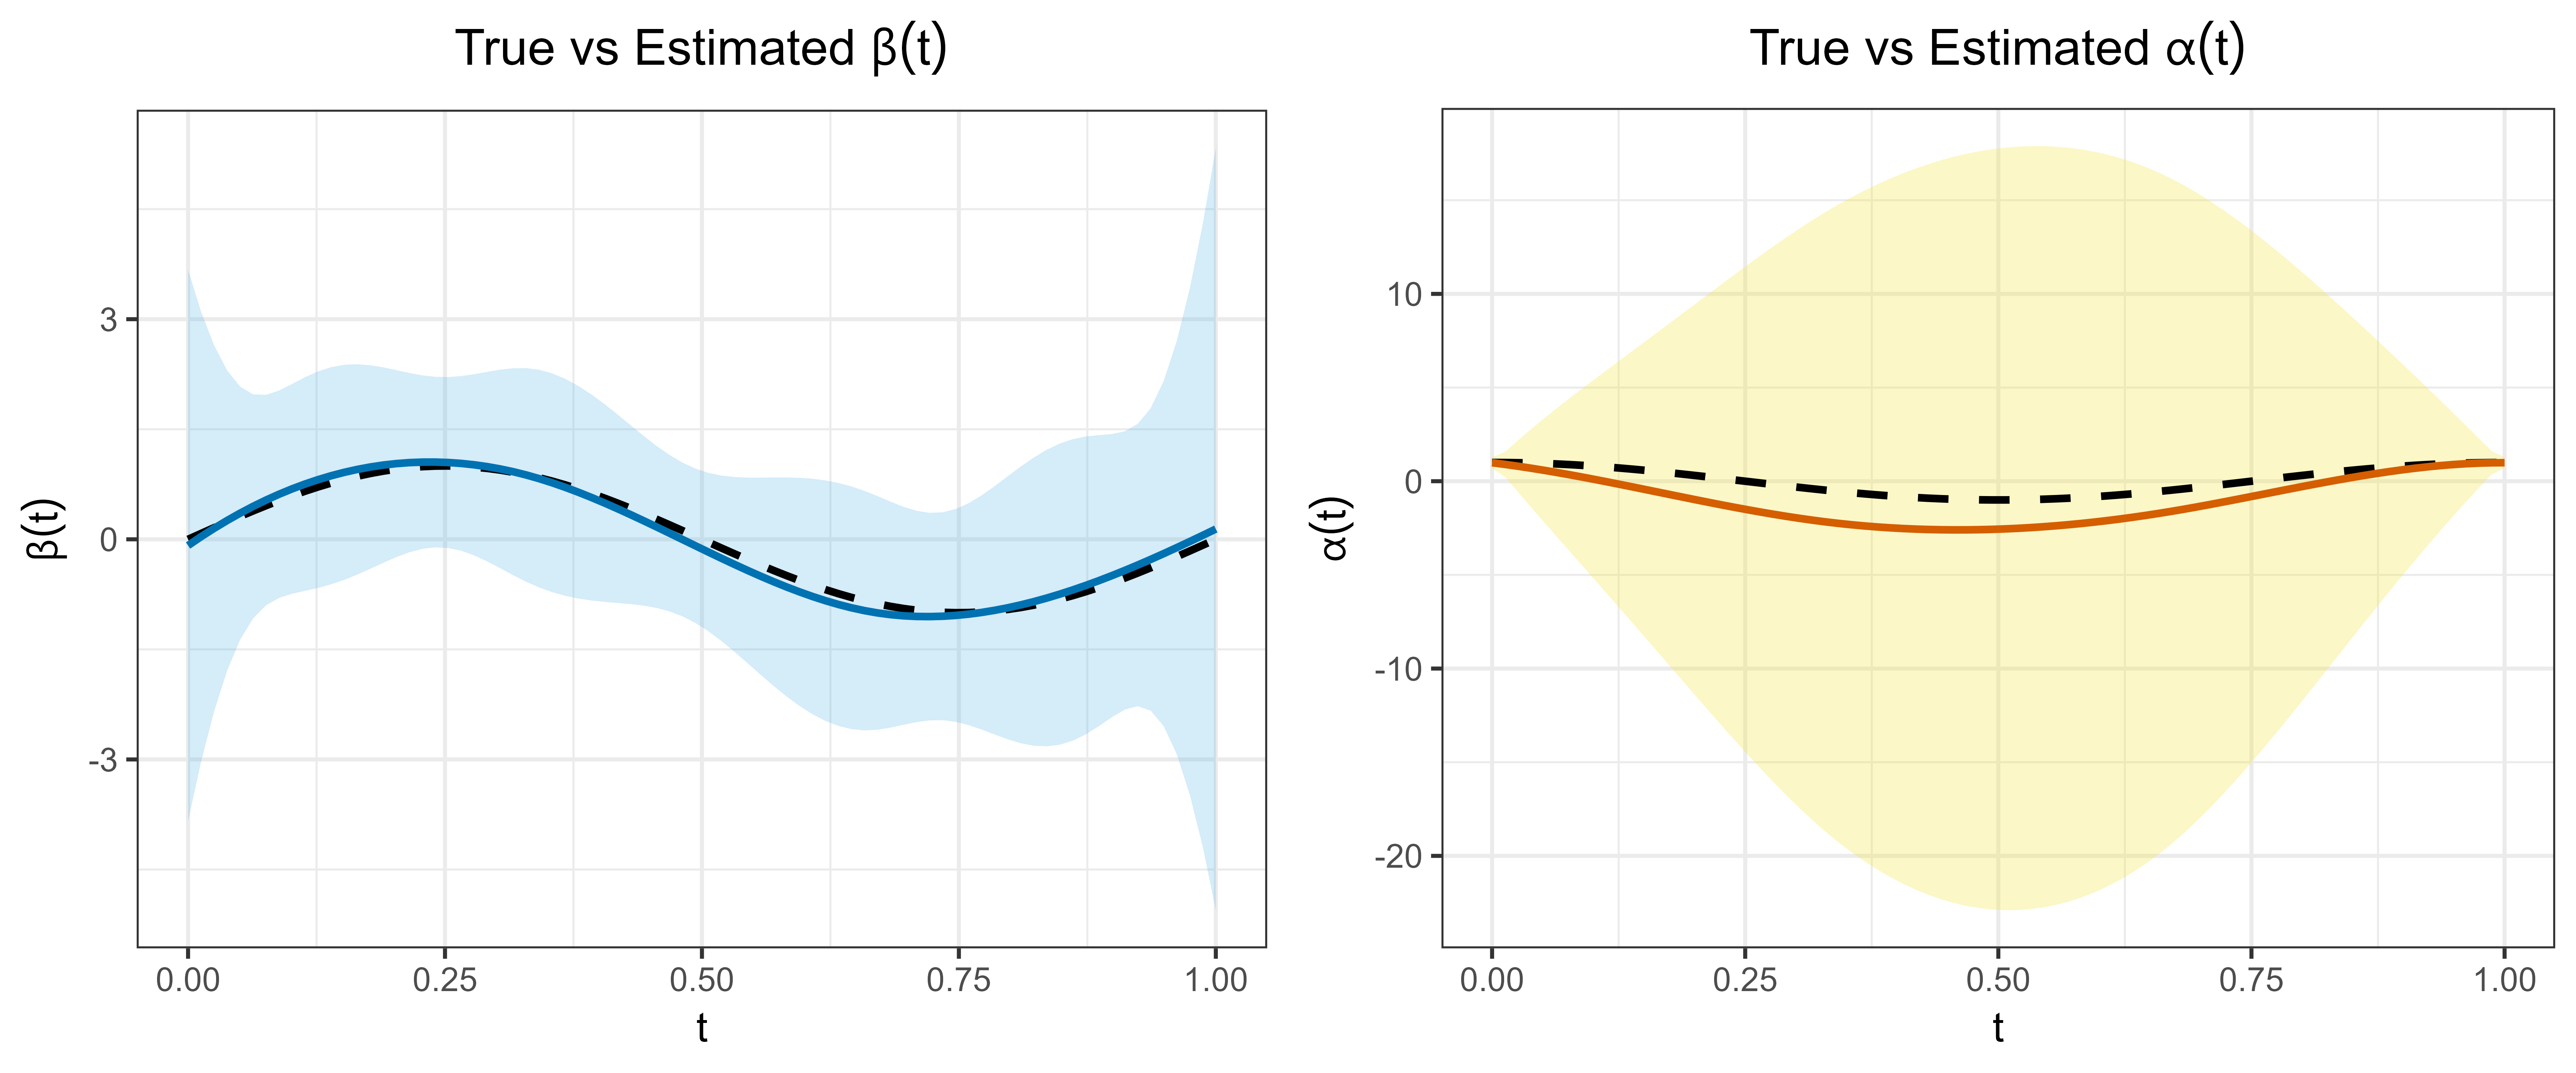
\includegraphics[width=0.85\linewidth]{Images/functional_coefficients.png}
		\caption{True and estimated functional coefficients with confidence bands.}
		\label{fig:coef_plot}
	\end{figure}
	
	\section{Real data application}
	
	We apply the proposed method to near-infrared (NIR) spectroscopy data from milk samples. The response variable is bounded in $(0,1)$, making beta regression an appropriate modeling choice. Each observation consists of a smooth absorbance spectrum measured over wavelengths together with scalar explanatory variables.
	
	\begin{figure}[H]
		\centering
		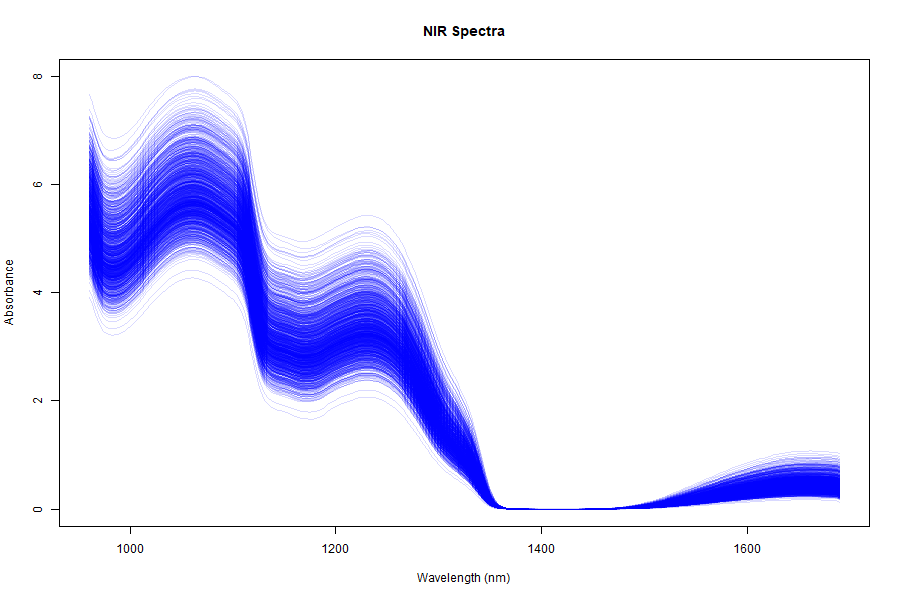
\includegraphics[width=0.85\linewidth]{Images/NIR_spectra.png}
		\caption{Smoothed NIR spectra of the milk samples.}
		\label{fig:nir}
	\end{figure}
	
	The spectra are first smoothed and then expanded using a basis representation. Their derivatives are computed numerically and included in the model. The fitted functional coefficients indicate that both the overall spectral shape and local changes in slope contribute to the response.
	
	The derivative effect is particularly useful in regions where the spectral curve changes rapidly. In these zones, the derivative provides crucial information that significantly reduces predictive error.
	
	\begin{figure}[H]
		\centering
		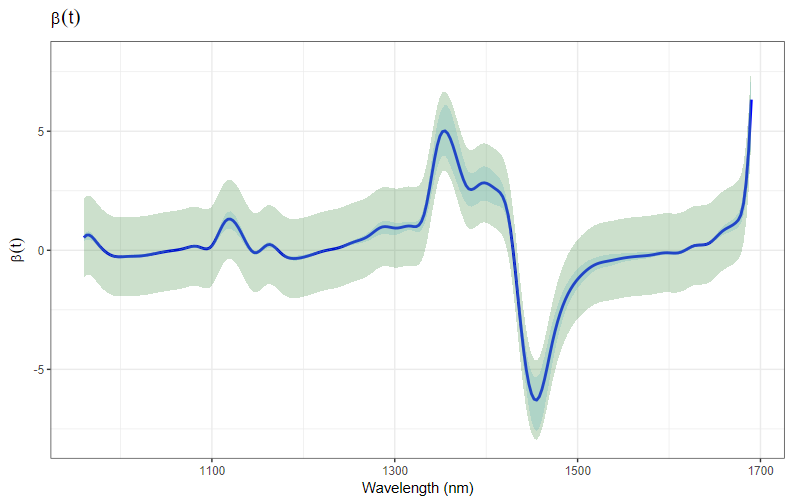
\includegraphics[width=0.85\linewidth]{Images/plot6.png}
		\caption{Estimated functional coefficient with bootstrap confidence bands.}
		\label{fig:real_coef}
	\end{figure}
	
\section{Discussion and conclusion}

In this paper, we introduced a partial functional beta regression model that effectively incorporates both functional predictors and their derivative information. By utilizing basis expansions and penalized likelihood estimation, the model captures complex dynamic behaviors in bounded response data, which are often missed by standard functional models.

Our theoretical results established the identifiability and consistency of the estimators, while simulation studies and real-data application to NIR spectroscopy confirmed a significant reduction in predictive error (RMSE and MAE). The inclusion of derivative terms proved particularly beneficial in spectral regions with rapid changes, providing better interpretability and predictive power. Future research could extend this framework to handle sparse functional data or incorporate non-parametric penalty selection.

	\begin{thebibliography}{99}
		\bibitem[Cardot et~al.(1999)]{Cardot1999} Cardot, H., Ferraty, F., and Sarda, P. (1999). Functional linear model. \emph{Statist. Probab. Lett.}, 45, 11-22.
		\bibitem[Di Brisco et~al.(2023)]{DiBrisco2023} Di Brisco, A., et al. (2023). Bayesian flexible beta regression model with functional covariate. \emph{Computational Statistics}.
		\bibitem[Ferrari and Cribari-Neto(2004)]{FerrariCribari2004} Ferrari, S., and Cribari-Neto, F. (2004). Beta regression. \emph{J. Appl. Stat.}, 31, 799-815.
		\bibitem[Hall and Hooker(2016)]{HallHooker2016} Hall, P., and Hooker, G. (2016). Derivative order selection. \emph{Ann. Statist.}, 44, 2526-2550.
		\bibitem[Hooker and Shang(2020)]{HookerShang2020} Hooker, G., and Shang, H. (2020). Selecting derivatives in functional regression. \emph{Journal of Computational and Graphical Statistics}.
		\bibitem[Ramsay and Silverman(2005)]{RamsaySilverman2005} Ramsay, J., and Silverman, B. W. (2005). \emph{Functional Data Analysis}. Springer.
	\end{thebibliography}
	
\end{document}
